\documentclass[a4paper,12pt]{article}
\usepackage{a4wide}
\usepackage{graphicx}
\graphicspath{{.}}

\begin{document}

	
	\title{Tema Curs 6 Baze de Date}
	\author{Moroianu Theodor (135)}
	\date{\today}
	\maketitle

	\section{Diagrama Relationala\newline}
	
	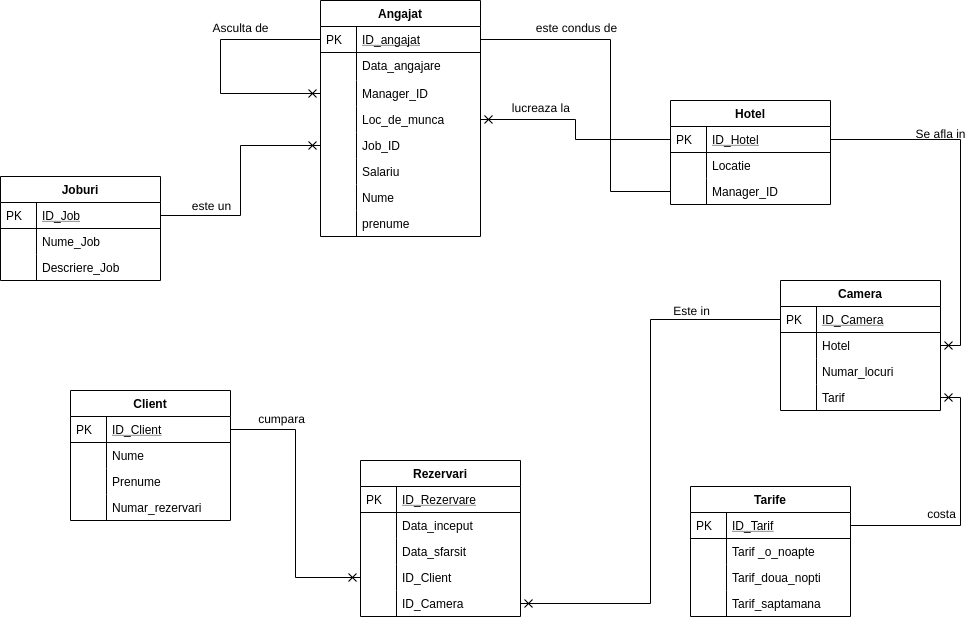
\includegraphics[scale=0.5]{diagrama_tema_6_curs.png}
	
	\newpage
	
	\section{Scheme Relationale}
	
	\begin{itemize}
		\item \textbf{Angajat:} \underline{ID\_ANGAJAT}, Data\_angajare, Manager\_ID, Loc\_de\_munca, Job\_ID, Salariu
		\item \textbf{Client:} \underline{ID\_Client}, Nume, Prenume, Numar\_rezervari
		\item \textbf{Joburi:} \underline{ID\_Job}, Nume\_Job, Descriere\_Job
		\item \textbf{Rezervari:} \underline{ID\_Rezervare}, Data\_inceput, Data\_sfarsit, ID\_Client, ID\_Camera
		\item \textbf{Camera:} \underline{ID\_Camera}, Hotel, Numar\_locuri, Tarif
		\item \textbf{Tarife:} \underline{ID\_Tarif}, Tarif\_o\_noapte, Tarif\_doua\_nopti, Tarif\_saptamana
		\item \textbf{Hotel:} \underline{ID\_Hotel}, Locatie, Manager\_ID
	\end{itemize}
	
	\section{Extemple de operatii algebrice relationale}
	
	\subsection{}
		\textit{Să se afişeze clienţii (codul şi numele acestora) în ordine alfabetică a numelor, din statele IN, OH, MI, IL şi ale căror nume încep cu literele A sau B.\\}
		\textbf{Raspuns:\\SELECT cust\_id, cust\_name\\
			FROM customer\_TBL\\
			WHERE SUBSTR(UPPER(cust\_name), 1, 1) IN ('A', 'B') AND cust\_state IN ('IN', 'OH', 'MI', 'IL')\\ 
			ORDER BY cust\_name;}
	
	\subsection{}
	\begin{itemize}
	\item[a)] \emph{Să se obţină codul, descrierea şi costul produselor a căror valoare se situează între 1 şi 12.50.\\}
	\textbf{Raspuns:\\SELECT prod\_id, prod\_desc, cost\\
		FROM products\_tbl\\
		WHERE cost BETWEEN 1 AND 12.50;\\}
	
	\item[b)] \emph{Să se obţină codul, descrierea şi costul produselor a căror valoare este mai mică decât 1 sau mai mare decât 12.50.\\}
	\textbf{Raspuns:\\SELECT prod\_id, prod\_desc, cost\\
		FROM products\_tbl\\
		WHERE cost NOT BETWEEN 1 AND 12.50;\\}
	\end{itemize}
	
	\subsection{}
	\textit{Să se listeze adresele de email ale angajaţilor. Acestea au următoarea formă:
		first\_name.last\_name@ittech.com.\\}
	\textbf{Raspuns:\\
		SELECT LOWER(first\_name) $||$ '.' $||$ LOWER(last\_name) $||$ '@ittech.com' as "mail"\\
		FROM employee\_tbl\\
		ORDER BY "mail";}
	
	\subsection{}
	\textit{Să se afişeze, pentru fiecare angajat, numele, codul şi numărul de telefon în
		formatele următoare:\\NAME = SMITH, JOHN\\
		EMP\_ID = 999-99-9999\\
		PHONE = (999)999-9999\\}
	\textbf{Raspuns:\\
		SELECT 'NAME = ' $||$ last\_name $||$ ', ' $||$ first\_name $||$ '   '
		$||$ 'EMP\_ID = ' $||$ SUBSTR(emp\_id, 0, 3) $||$ '-' $||$ SUBSTR(emp\_id, 3, 2) $||$ '-' $||$ SUBSTR(emp\_id, 5, 4) $||$ '   '
		$||$ 'PHONE = (' $||$ SUBSTR(phone, 0, 3) $||$ ')' $||$ SUBSTR(phone, 3, 3) $||$ '-' $||$ SUBSTR(phone, 6, 4) $||$ '   '
		as "Employee"\\
		FROM employee\_TBL;\\}
	
	\subsection{}
	\textit{Să se afişeze codul şi anul angajării salariaţilor din firmă.\\}
	\textbf{Raspuns:\\
	SELECT emp\_id, TO\_CHAR(date\_hire, 'YYYY') as "An"\\
	FROM employee\_pay\_tbl;}
	
	\subsection{}
	\textit{Să se determine codul, numele, prenumele, salariul şi bonusul angajaţilor.\\}
	\textbf{Raspuns:\\SELECT emp.emp\_id, emp.last\_name, pay.salary, pay.bonus\\
		FROM employee\_tbl emp LEFT JOIN employee\_pay\_tbl pay\\
		ON emp.emp\_id = pay.emp\_id;}
	
	\subsection{}
	\textit{Să se afişeze numele clienţilor, codurile comenzilor şi data la care au fost lansate, pentru clienţii din statele al căror cod începe cu litera "I".\\}
	\textbf{Raspuns:\\SELECT c.cust\_name, o.ord\_num, o.ord\_date\\
		FROM orders\_tbl o JOIN customer\_tbl c ON o.cust\_id = c.cust\_id\\
		WHERE UPPER(c.cust\_state) LIKE 'I\%';}
	
	\subsection{}
	\textit{Să se obţină informaţii despre comenzi (număr, cantitate) şi angajaţii care au preluat acele comenzi (nume, prenume, oraş).\\}
	\textbf{Raspuns:\\SELECT o.ord\_num, o.qty, e.first\_name, e.last\_name, e.city\\
		FROM orders\_tbl o JOIN employee\_tbl e ON o.sales\_rep = e.emp\_id;}
	
	\subsection{}
	\textit{Se cer informaţiile de la exerciţiul precedent, afişându-se în plus şi angajaţii care nu au preluat nicio comandă.\\}
	\textbf{Raspuns:\\SELECT o.ord\_num, o.qty, e.first\_name, e.last\_name, e.city\\
		FROM orders\_tbl o FULL JOIN employee\_tbl e ON o.sales\_rep = e.emp\_id;}
	
	\subsection{}
	\textit{Să se afişeze angajaţii pentru care valoarea câmpului middle\_name este necunoscută.\\}
	\textbf{Raspuns:\\SELECT *\\
		FROM employee\_tbl\\
		WHERE middle\_name is NULL;}
	
	\subsection{}
	\textit{Să se obţină salariul anual al angajaţilor, ţinând cont de bonus (se vor trata corespunzător valorile NULL!).\\}
	\textbf{Raspuns:\\
	SELECT emp\_id, NVL(salary, 0) * 12 + NVL(bonus, 0)\\
	FROM employee\_pay\_tbl;}
	
	\subsection{}
	\textit{Să se afişeze numele, salariul, poziţia şi o coloană etichetată "Salariu modificat" reprezentând salariul mărit cu 10\%, respectiv 15\% pentru angajaţii ocupând poziţii de marketing sau salesman. Pentru celelalte poziţii, coloana va afişa salariul nemodificat. Se cer 2 variante de rezolvare.\\}
	\textbf{Raspuns:\\}
	
	\begin{itemize}
		\item[a)] \textbf{SELECT e.last\_name, p.salary, p.position,
			(CASE 
			WHEN LOWER(p.position) = 'marketing' THEN 1.10
			WHEN LOWER(p.position) = 'salesman' THEN 1.15
			ELSE 1.0
			END) * p.salary as "Salariu modificat"
			FROM employee\_tbl e LEFT JOIN employee\_pay\_tbl p ON e.emp\_id = p.emp\_id;\\}
		
		\item[b)] \textbf{SELECT e.last\_name, p.salary, p.position, 
			DECODE(LOWER(p.position), 'marketing', 1.10,
			'salesman', 1.15,
			1.0) * p.salary as "Salariu Modificat"
			FROM employee\_tbl e LEFT JOIN employee\_pay\_tbl p ON e.emp\_id = p.emp\_id;}
	\end{itemize}

\end{document}